\documentclass[10pt,aspectratio=169,t]{beamer}

\usepackage[T1]{fontenc}
\usepackage[scaled=0.94]{helvet}
\renewcommand{\familydefault}{\sfdefault}
\usepackage{amsmath}
\usepackage{array}
\usepackage{booktabs}
\usepackage{graphicx}
\usepackage{tabularx}
\usepackage{tikz}
\usepackage{xcolor}
\usepackage{hyperref}
\usetikzlibrary{arrows.meta,positioning}

\definecolor{TTURed}{HTML}{CC0000}
\definecolor{CMSBlue}{HTML}{1F77B4}
\definecolor{CMSGreen}{HTML}{2CA02C}
\definecolor{CMSOrange}{HTML}{FF7F0E}
\definecolor{CMSGray}{HTML}{6B7280}
\definecolor{LightGray}{HTML}{E5E7EB}
\definecolor{DarkInk}{HTML}{111111}

\hypersetup{colorlinks=true,urlcolor=CMSBlue,linkcolor=DarkInk}
\setbeamertemplate{navigation symbols}{}
\setbeamercolor{normal text}{fg=DarkInk,bg=white}
\setbeamercolor{frametitle}{fg=black,bg=white}
\setbeamercolor{structure}{fg=TTURed}
\setbeamerfont{frametitle}{size=\fontsize{21}{23},series=\bfseries}
\setbeamerfont{normal text}{size=\fontsize{14}{17}}
\setbeamersize{text margin left=0.52cm,text margin right=0.52cm}

\setbeamertemplate{headline}{%
  \leavevmode%
  \begin{beamercolorbox}[wd=\paperwidth,ht=0.26cm,dp=0.02cm,rightskip=0.28cm]{structure}%
    \hfill\includegraphics[height=0.20cm]{assets/ttu_wordmark_white.png}%
  \end{beamercolorbox}%
  \begin{beamercolorbox}[wd=\paperwidth,ht=0.055cm,dp=0cm]{structure}\end{beamercolorbox}%
}
\setbeamertemplate{frametitle}{%
  \vspace{0.11cm}\insertframetitle\par\vspace{0.04cm}%
}
\setbeamertemplate{footline}{%
  \begin{beamercolorbox}[wd=\paperwidth,ht=0.045cm,dp=0cm,leftskip=0.33cm,rightskip=0.33cm]{normal text}%
    {\color{TTURed}\rule{0.955\paperwidth}{0.045cm}}%
  \end{beamercolorbox}%
  \hbox{%
    \begin{beamercolorbox}[wd=.27\paperwidth,ht=2.2ex,dp=.75ex,leftskip=.38cm]{normal text}%
      \fontsize{6.2}{7.0}\selectfont 20 Oct. 2026
    \end{beamercolorbox}%
    \begin{beamercolorbox}[wd=.54\paperwidth,ht=2.2ex,dp=.75ex,center]{normal text}%
      \fontsize{6.2}{7.0}\selectfont Chris Madrid $\mid$ CPAD 2026
    \end{beamercolorbox}%
    \begin{beamercolorbox}[wd=.19\paperwidth,ht=2.2ex,dp=.75ex,rightskip=.38cm plus1fil]{normal text}%
      \hfill\fontsize{6.2}{7.0}\selectfont\insertframenumber
    \end{beamercolorbox}%
  }%
}

\newcommand{\source}[1]{%
  \begin{tikzpicture}[remember picture,overlay]
    \node[anchor=south west,text width=0.91\paperwidth,align=left]
      at ([xshift=0.52cm,yshift=0.54cm]current page.south west)
      {\fontsize{5.5}{6.2}\selectfont\color{CMSGray}#1};
  \end{tikzpicture}%
}
\newcommand{\red}[1]{\textcolor{TTURed}{\bfseries #1}}
\newcommand{\blue}[1]{\textcolor{CMSBlue}{\bfseries #1}}
\newcommand{\green}[1]{\textcolor{CMSGreen}{\bfseries #1}}
\newcommand{\tightitem}{\setlength\itemsep{0.33em}\setlength\parskip{0pt}}
\newcommand{\flatbox}[2]{%
  \begin{tikzpicture}
    \node[draw=#1,line width=1.2pt,inner sep=5pt,align=center,text width=0.93\linewidth] {#2};
  \end{tikzpicture}%
}

\title{FLASH: photon-level time-resolved calorimetry with digital SiPMs}
\author{Chris Madrid}
\institute{Texas Tech University $\mid$ SLAC LDRD collaboration}
\date{CPAD 2026 $\mid$ Seattle}

\begin{document}

% 1
\begin{frame}[plain]
  \vspace{0.72cm}
  {\fontsize{26}{30}\selectfont\bfseries
    FLASH: photon-level time-resolved\\[0.08cm]
    calorimetry with digital SiPMs\par}
  \vspace{0.38cm}
  {\fontsize{15}{18}\selectfont
    What happens if HG-DREAM is read out as sparse photon hits?\par}
  \vfill
  \begin{columns}[b,onlytextwidth]
    \begin{column}{0.18\textwidth}
      \includegraphics[height=1.45cm]{assets/particle_detector_lab.jpeg}
    \end{column}
    \begin{column}{0.80\textwidth}
      {\fontsize{14}{17}\selectfont\bfseries Chris Madrid\par}
      {\fontsize{10.5}{13}\selectfont Texas Tech University $\mid$ SLAC LDRD collaboration\par}
      \vspace{0.09cm}
      {\fontsize{10.5}{13}\selectfont CPAD 2026, Seattle $\mid$ 20 October 2026\par}
    \end{column}
  \end{columns}
  \vspace{0.25cm}
\end{frame}

% 2
\begin{frame}{The detector question is more important than the sensor question}
  \vspace{0.22cm}
  \centering
  {\fontsize{23}{27}\selectfont\bfseries
    If HG-DREAM were read out with dSiPMs,\\
    which calorimeter information would survive?\par}
  \vspace{0.36cm}
  \begin{columns}[T,onlytextwidth]
    \begin{column}{0.31\textwidth}
      \flatbox{TTURed}{\large\bfseries Energy\\[0.08cm]\normalsize linearity, resolution, $C/S$}
    \end{column}
    \begin{column}{0.31\textwidth}
      \flatbox{CMSBlue}{\large\bfseries Imaging\\[0.08cm]\normalsize shower core, transverse shape}
    \end{column}
    \begin{column}{0.31\textwidth}
      \flatbox{CMSGreen}{\large\bfseries Timing\\[0.08cm]\normalsize depth, pileup, sparse data}
    \end{column}
  \end{columns}
  \vspace{0.22cm}
  \raggedright\small
  The specification is not ``10--50 ps.'' It is the \red{joint operating point} in PDE, pitch, recovery, timing architecture, and output format that preserves these observables.
\end{frame}

% 3
\begin{frame}{Why HG-DREAM is the right benchmark}
  \begin{columns}[T,onlytextwidth]
    \begin{column}{0.52\textwidth}
      \includegraphics[width=\linewidth,height=0.67\textheight,keepaspectratio]{assets/hgdream_detector_photo.png}
    \end{column}
    \begin{column}{0.45\textwidth}
      \vspace{0.08cm}
      \begin{itemize}\tightitem
        \item \red{Real optical density}: electromagnetic cores stress recovery and dynamic range.
        \item \blue{Two observables}: Cherenkov and scintillation signals constrain hadronic fluctuations.
        \item \green{Measured reference}: 2025--26 beam data provide the closure target.
        \item Fine transverse segmentation and fast waveforms make the information loss testable.
      \end{itemize}
      \vspace{0.20cm}
      \flatbox{TTURed}{\bfseries HG-DREAM converts a device study into a calorimeter study.}
    \end{column}
  \end{columns}
  \source{HG-DREAM photo and detector description: Y. Feng, CALOR 2026; C. Madrid, Higgs 2025.}
\end{frame}

% 4
\begin{frame}{The replacement changes what one channel reports}
  \vspace{0.20cm}
  \begin{columns}[T,onlytextwidth]
    \begin{column}{0.45\textwidth}
      {\large\bfseries Current HG-DREAM chain}\par
      \vspace{0.16cm}
      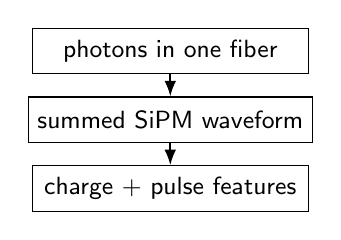
\begin{tikzpicture}[node distance=0.28cm,every node/.style={font=\small,minimum width=3.5cm,minimum height=.58cm}]
        \node[draw=black] (a) {photons in one fiber};
        \node[draw=black,below=of a] (b) {summed SiPM waveform};
        \node[draw=black,below=of b] (c) {charge + pulse features};
        \draw[-{Latex[length=2mm]},thick] (a)--(b);
        \draw[-{Latex[length=2mm]},thick] (b)--(c);
      \end{tikzpicture}
      \vspace{0.15cm}

      \small The event keeps the integrated optical response and selected waveform observables.
    \end{column}
    \begin{column}{0.07\textwidth}
      \centering\vspace{1.28cm}{\Large$\Longrightarrow$}
    \end{column}
    \begin{column}{0.45\textwidth}
      {\large\bfseries FLASH dSiPM chain}\par
      \vspace{0.16cm}
      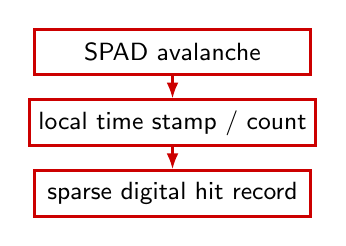
\begin{tikzpicture}[node distance=0.28cm,every node/.style={font=\small,minimum width=3.5cm,minimum height=.58cm}]
        \node[draw=TTURed,line width=1.1pt] (a) {SPAD avalanche};
        \node[draw=TTURed,line width=1.1pt,below=of a] (b) {local time stamp / count};
        \node[draw=TTURed,line width=1.1pt,below=of b] (c) {sparse digital hit record};
        \draw[-{Latex[length=2mm]},thick,TTURed] (a)--(b);
        \draw[-{Latex[length=2mm]},thick,TTURed] (b)--(c);
      \end{tikzpicture}
      \vspace{0.15cm}

      \small The event can keep photon-level space--time information, but finite cells and recovery reshape the signal.
    \end{column}
  \end{columns}
  \vspace{0.35cm}
  \centering\red{The calorimeter geometry is unchanged; the measurement operator is not.}
\end{frame}

% 5
\begin{frame}{The study now uses complete showers across the detector}
  \small
  \begin{columns}[T,onlytextwidth]
    \begin{column}{0.58\textwidth}
      \vspace{0.10cm}
      \fontsize{7.6}{9.0}\selectfont
      \begin{tabularx}{\linewidth}{>{\bfseries}l r r r}
        \toprule
        Sample & Events & C photons/event & active fibers/event \\
        \midrule
        100 GeV $e^+$ & 1000 & 13,749 & 841 \\
        90 GeV $\pi^+$ & 100 & 9,377 & 1,386 \\
        \bottomrule
      \end{tabularx}
      \vspace{0.38cm}
      \begin{itemize}\tightitem
        \item Absolute fiber endpoints are mapped to the repeated 4 mm rod lattice.
        \item Every photon is assigned to a physical fiber, local SPAD cell, and arrival time.
        \item PDE and recovery are applied independently in every physical sensor.
      \end{itemize}
    \end{column}
    \begin{column}{0.39\textwidth}
      \vspace{0.05cm}
      \includegraphics[width=\linewidth,height=0.53\textheight,keepaspectratio]{assets/hgdream_fiber_layout.png}
      \vspace{0.06cm}

      \fontsize{8}{10}\selectfont\color{CMSGray}
      Scope today: explicit optical photons are available for the Cherenkov side. The stored scintillation signal is retained but not yet photon-digitized.
    \end{column}
  \end{columns}
\end{frame}

% 6
\begin{frame}{Validation defines what may be compared}
  \centering
  \includegraphics[width=0.94\textwidth,height=0.70\textheight,keepaspectratio]{assets/full_detector_validation.png}
  \vspace{-0.08cm}

  \small The explicit photon count tracks the stored Cherenkov signal, but it is not the same observable: \blue{$r=0.73$} for electrons and \red{$r=0.90$} for pions.
  \source{DREAMSim full-detector samples; 0--40 ns Cherenkov photon selection.}
\end{frame}

% 7
\begin{frame}{A realistic dSiPM preserves the shower image}
  \centering
  \includegraphics[width=0.99\textwidth,height=0.76\textheight,keepaspectratio]{assets/full_detector_event_display.png}
  \vspace{-0.08cm}

  \small Representative 90 GeV pion: the global transverse image is stable; the recovery loss is localized to the shower core.
\end{frame}

% 8
\begin{frame}{Dynamic range is a local shower-core problem}
  \centering
  \includegraphics[width=0.94\textwidth,height=0.66\textheight,keepaspectratio]{assets/full_detector_occupancy.png}
  \vspace{-0.08cm}

  \parbox{0.94\textwidth}{\centering\fontsize{8.7}{10.2}\selectfont The median brightest fiber contains about \blue{621 photons} for a 100 GeV electron and \red{145 photons} for a 90 GeV pion. A single average occupancy cannot define the sensor.}
\end{frame}

% 9
\begin{frame}{The requirement is particle-dependent linearity, not apparent narrowing}
  \centering
  \includegraphics[width=0.93\textwidth,height=0.63\textheight,keepaspectratio]{assets/full_detector_performance_scan.png}
  \vspace{-0.05cm}

  \parbox{0.95\textwidth}{\centering\fontsize{8.7}{10.2}\selectfont At 20 $\mu$m and 4.3 ns, recovery keeps \blue{97.8\%} of detected electron photons and \red{99.4\%} for pions. Electron calibration therefore shifts the pion C response by \red{$+1.7\%$}. Coarser pixels narrow the distribution by saturation---not by adding information.}
\end{frame}

% 10
\begin{frame}{Event-level propagation makes the nonlinearity visible}
  \centering
  \includegraphics[width=0.93\textwidth,height=0.63\textheight,keepaspectratio]{assets/full_detector_response.png}
  \vspace{-0.02cm}

  \parbox{0.94\textwidth}{\centering\fontsize{8.7}{10.2}\selectfont Left: Cherenkov response after electron calibration. Right: an illustrative fixed-$\chi$ dual-readout propagation; it is deliberately shown as sensitivity, not a final resolution prediction.}
\end{frame}

% 11
\begin{frame}{What changed relative to the original study}
  \begin{columns}[T,onlytextwidth]
    \begin{column}{0.47\textwidth}
      {\large\bfseries The useful result}\par
      \begin{itemize}\tightitem
        \item The historical plots reproduce exactly as software closure.
        \item Dense Cherenkov fibers do probe pitch and recovery.
        \item Pulse-shape distortion starts before catastrophic count loss.
      \end{itemize}
    \end{column}
    \begin{column}{0.47\textwidth}
      {\large\bfseries The required correction}\par
      \begin{itemize}\tightitem
        \item A 3 mm sensor grid was drawn across a 1 mm fiber-local window.
        \item The labeled pitch was effectively divided by three.
        \item The corrected study uses physical millimeters and full showers.
      \end{itemize}
    \end{column}
  \end{columns}
  \vspace{0.38cm}
  \centering
  \flatbox{TTURed}{\bfseries Single-fiber retention is a diagnostic. Full-detector response transfer is the requirement.}
  \vspace{0.15cm}

  {\raggedright\fontsize{5.5}{6.2}\selectfont\color{CMSGray}Historical reference: C. Madrid and S. McKinley, ``Digital SiPM Light Occupancy Study,'' SLAC+TTU 5D Calorimetry, 30 Apr. 2025.\par}
\end{frame}

% 12
\begin{frame}{Timing remains the second half of the physics case}
  \begin{columns}[T,onlytextwidth]
    \begin{column}{0.58\textwidth}
      \vspace{0.15cm}
      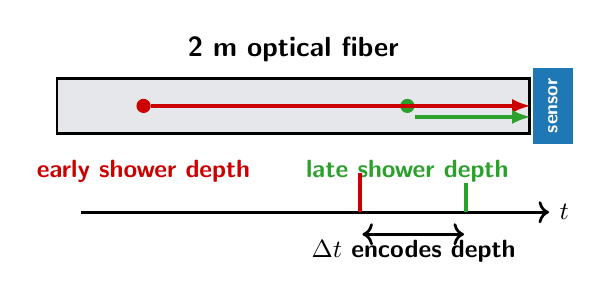
\begin{tikzpicture}[x=1cm,y=1cm]
        \draw[fill=LightGray,draw=black,line width=1.0pt] (0,1.55) rectangle (6.0,2.25);
        \node[anchor=south,font=\bfseries] at (3.0,2.34) {2 m optical fiber};
        \draw[fill=CMSBlue,draw=CMSBlue] (6.05,1.42) rectangle (6.55,2.38);
        \node[rotate=90,white,font=\bfseries\scriptsize] at (6.30,1.90) {sensor};
        \fill[TTURed] (1.1,1.90) circle (0.09);
        \fill[CMSGreen] (4.45,1.90) circle (0.09);
        \draw[-{Latex[length=2.4mm]},TTURed,line width=1.4pt] (1.2,1.90) -- (6.02,1.90);
        \draw[-{Latex[length=2.4mm]},CMSGreen,line width=1.4pt] (4.55,1.76) -- (6.02,1.76);
        \node[TTURed,anchor=north,font=\small\bfseries] at (1.1,1.34) {early shower depth};
        \node[CMSGreen,anchor=north,font=\small\bfseries] at (4.45,1.34) {late shower depth};
        \draw[->,line width=1pt] (0.30,0.55) -- (6.25,0.55) node[right,font=\small] {$t$};
        \draw[TTURed,line width=1.5pt] (3.85,0.55) -- (3.85,1.05);
        \draw[CMSGreen,line width=1.5pt] (5.20,0.55) -- (5.20,0.92);
        \draw[<->,line width=1pt] (3.88,0.27) -- (5.17,0.27);
        \node[font=\small\bfseries] at (4.53,0.05) {$\Delta t$ encodes depth};
      \end{tikzpicture}
      \vspace{0.10cm}

      \centering\small Arrival time combines shower production time and optical transport.
    \end{column}
    \begin{column}{0.39\textwidth}
      \vspace{0.10cm}
      \begin{itemize}\tightitem
        \item Fiber transport maps production depth into arrival time.
        \item Shower and optical dispersion already dominate simple depth proxies.
        \item Fine TDC bins alone do not guarantee fine calorimeter depth resolution.
      \end{itemize}
      \vspace{0.18cm}
      \flatbox{CMSBlue}{\bfseries Next: compare matched analog waveforms and sparse timestamps on the same full-detector events.}
    \end{column}
  \end{columns}
  \source{Y. Feng, CALOR 2026, longitudinal segmentation with timing; FLASH simulation audit.}
\end{frame}

% 13
\begin{frame}{FLASH is an architecture space, not one number}
  \small
  \begin{tabularx}{\textwidth}{>{\bfseries}l >{\raggedright\arraybackslash}X >{\raggedright\arraybackslash}X}
    \toprule
    Design choice & Physics consequence & LDRD measurement / decision \\
    \midrule
    PDE$(\lambda)$ & photon statistics and C/S response & spectral PDE on candidate SPAD tier \\
    SPAD pitch + recovery & particle-dependent saturation & bright-pulse and double-pulse scans \\
    timing-group size & depth information vs area/power & first-hit, multi-hit, and histogram modes \\
    SPTR + TDC & timestamp precision & separate sensor IRF from TDC binning \\
    output policy & sparse-data value and bandwidth & event payload under realistic showers \\
    masking / DCR / cross-talk & bias and fake-hit rate & measured maps inserted into simulation \\
    \bottomrule
  \end{tabularx}
  \vspace{0.30cm}
  \centering\red{The prototype program should close this table one row at a time.}
\end{frame}

% 14
\begin{frame}{The next simulation set should close the calorimeter loop}
  \begin{enumerate}\tightitem
    \item \red{Generate matched full-detector samples} with explicit Cherenkov and scintillation photons in one configuration.
    \item \red{Run an energy scan} for $e^+$ and $\pi^+$ so linearity and stochastic terms replace single-energy response widths.
    \item \blue{Digitize current and FLASH readouts} from the same photons, including PDE$(\lambda)$, DCR, cross-talk, afterpulsing, recovery, and masks.
    \item \blue{Reconstruct the same observables}: $S$, $C$, dual-readout energy, transverse moments, timing depth, and particle ID.
    \item \green{Report an information/performance frontier}: physics resolution versus power, active area, and event payload.
  \end{enumerate}
  \vspace{0.28cm}
  \flatbox{TTURed}{\bfseries Decision criterion: choose the simplest FLASH architecture that reproduces the HG-DREAM observables and adds useful timing.}
\end{frame}

% 15
\begin{frame}{What the present result already tells the LDRD}
  \begin{columns}[T,onlytextwidth]
    \begin{column}{0.31\textwidth}
      \flatbox{CMSBlue}{\fontsize{20}{22}\selectfont\bfseries 20 $\mu$m\\[0.08cm]\normalsize viable working point, not yet a requirement}
    \end{column}
    \begin{column}{0.31\textwidth}
      \flatbox{CMSGreen}{\fontsize{20}{22}\selectfont\bfseries 4.3 ns\\[0.08cm]\normalsize modest aggregate loss in these samples}
    \end{column}
    \begin{column}{0.31\textwidth}
      \flatbox{TTURed}{\fontsize{20}{22}\selectfont\bfseries $+1.7\%$\\[0.08cm]\normalsize pion C shift after electron calibration}
    \end{column}
  \end{columns}
  \vspace{0.50cm}
  \begin{itemize}\tightitem
    \item The spatial shower image survives at this point.
    \item The important failure mode is \red{differential saturation between particles}, not an average hit-loss threshold.
    \item The next design decision needs energy scans and matched C/S photon simulation.
  \end{itemize}
\end{frame}

% 16
\begin{frame}{Conclusions}
  \vspace{0.20cm}
  \begin{itemize}\setlength\itemsep{0.60em}
    \item \red{HG-DREAM is the benchmark}: it tests energy, imaging, timing, and real photon density together.
    \item We now propagate dSiPM pitch, PDE, and recovery through \blue{complete detector showers}.
    \item A 20 $\mu$m, 4.3 ns point preserves the transverse image, but electron/pion occupancy differences create a measurable response transfer.
    \item The CPAD claim should be: \green{FLASH is being designed against calorimeter observables, not isolated device specifications.}
  \end{itemize}
  \vfill
  \centering{\large\bfseries Next milestone: matched full-detector C/S samples $\rightarrow$ energy scan $\rightarrow$ prototype closure.}
\end{frame}

\appendix

% 17
\begin{frame}{Backup: full-detector input audit}
  \small
  \begin{tabularx}{\textwidth}{>{\bfseries}l r r r r}
    \toprule
    Sample & events & C photons/event & active fibers/event & hottest fiber median \\
    \midrule
    100 GeV $e^+$ & 1000 & 13,749 & 841 & 621 \\
    90 GeV $\pi^+$ & 100 & 9,377 & 1,386 & 145 \\
    \bottomrule
  \end{tabularx}
  \vspace{0.34cm}
  \begin{itemize}\tightitem
    \item Selection: valid fiber index, Cherenkov core, positive sensor-plane exit, 0--40 ns gate, finite coordinates.
    \item Full geometry: four local fiber centers repeated on the 4 mm rod lattice.
    \item The 3 mm sensor fully contains the simulated fiber-core endpoints.
  \end{itemize}
\end{frame}

% 18
\begin{frame}{Backup: stored C and explicit photons must not be mixed silently}
  \centering
  \includegraphics[width=0.91\textwidth,height=0.64\textheight,keepaspectratio]{assets/full_detector_validation.png}
  \parbox{0.93\textwidth}{\centering\fontsize{8.7}{10.2}\selectfont The response scan uses a PDE-only explicit-photon baseline. The stored $S+C$ response remains a separate reference until matched production is available.}
\end{frame}

% 19
\begin{frame}{Backup: the historical pitch labels were effectively three times finer}
  \centering
  \includegraphics[width=0.83\textwidth,height=0.65\textheight,keepaspectratio]{assets/v2_mapping_correction.png}
  \small Reproduction closes the old software; the corrected physical map defines the new requirement study.
  \par\vspace{0.04cm}
  {\raggedright\fontsize{5.5}{6.2}\selectfont\color{CMSGray}Original sequence and pitch labels: C. Madrid and S. McKinley, Digital SiPM Light Occupancy Study (2025).\par}
\end{frame}

% 20
\begin{frame}{Backup: the one-fiber requirement remains a useful stress test}
  \centering
  \includegraphics[width=0.84\textwidth,height=0.69\textheight,keepaspectratio]{assets/v2_physical_requirements.png}
  \small At 20\% PDE and 4.3 ns recovery, a 20 $\mu$m pitch retains about 92.7\% of detected photons in the selected 1 TeV-pion fiber sample.
\end{frame}

% 21
\begin{frame}{Backup: recovery reshapes the pulse}
  \centering
  \includegraphics[width=0.86\textwidth,height=0.70\textheight,keepaspectratio]{assets/v2_pulse_shape.png}
  \small The prompt peak is preferentially suppressed, so timing and energy observables must be validated together.
\end{frame}

% 22
\begin{frame}{Backup: public timing numbers answer different questions}
  \centering
  \includegraphics[width=0.90\textwidth,height=0.70\textheight,keepaspectratio]{assets/timing_landscape.png}
  \small SPTR, photon-response IRF, TDC binning, and exported timestamp policy are not interchangeable specifications.
\end{frame}

% 23
\begin{frame}{Backup: what every headline plot is meant to establish}
  \fontsize{8.0}{9.6}\selectfont
  \begin{tabularx}{\textwidth}{>{\bfseries}p{3.2cm} X X}
    \toprule
    Plot & Question & Intended statement \\
    \midrule
    Full-detector validation & Are the photon and stored C branches interchangeable? & Correlated, not identical; keep baselines separate. \\
    Event display & Does the image survive? & Yes at the 20 $\mu$m / 4.3 ns point; losses localize in the core. \\
    Occupancy & Where is the stress? & The brightest fiber, not the event average, drives recovery. \\
    Sensor scan & What sets the requirement? & Particle-dependent response transfer, not apparent narrowing. \\
    Response propagation & Does a small C shift matter? & It can be amplified by a dual-readout estimator; validate with matched C/S samples. \\
    \bottomrule
  \end{tabularx}
\end{frame}

\end{document}
